\documentclass[sigconf]{acmart}

\usepackage{graphicx}
\usepackage{hyperref}
\usepackage{todonotes}

\usepackage{endfloat}
\renewcommand{\efloatseparator}{\mbox{}} % no new page between figures

\usepackage{booktabs} % For formal tables

\settopmatter{printacmref=false} % Removes citation information below abstract
\renewcommand\footnotetextcopyrightpermission[1]{} % removes footnote with conference information in first column
\pagestyle{plain} % removes running headers

\newcommand{\TODO}[1]{\todo[inline]{#1}}

\begin{document}
\title{Using Big Data to Battle Air Pollution}

\author{Karthik Vegi}
\affiliation{%
  \institution{Indiana University Bloomington}
  \streetaddress{2619 East 2nd Street, Apt 11}
  \city{Bloomington, IN 47401} 
  \country{USA}}
\email{kvegi@iu.com}


% The default list of authors is too long for headers}
\renewcommand{\shortauthors}{kvegi}


\begin{abstract}
We have come a long way from the stone age to build large scale industries, big cities, bullet trains, and a booming automobile industry. Technological and industrial advances are making our cities smarter by the day and yet a nagging side-effect is air pollution. Air pollution is not only creating local health hazards like respiratory and heart problems, but also directly leading to an increase in temperatures and contributing to global warming. We show how the advances in {\em Big Data}, {\em Cloud Computing}, and {\em Internet Of Devices} can be used to combat air pollution.
\end{abstract}

\keywords{i523, hid231, big data, environment, air pollution, global warming}

\maketitle

\section{Introduction}
Air pollution is no longer a local problem. It is a global environmental issue which involves individual countries to come together and device measures to combat it \cite{www-ral}. It it causing about 3.7 million premature deaths worldwide from cardiovascular and respiratory diseases and also ruins the crops that feed the world \cite{www-ral}. Air pollution also has a direct effect on a number of environmental issues like global warming, depletion of ozone layer, acid rains and impacts wild-life \cite{www-ral}. \\
Back in the year 1990, the job of a typical air quality scientist was to develop atmospheric dispersion models to evaluate the air pollution caused by industries and make sure that it is within the permissible level suggested by the {\em Environmental Protection Agency} \cite{www-ibm1}. These models gather historic data of many years from airports and weather balloons to predict the pollution with the help of meteorology theory \cite{www-ibm1}. Although the methods used to derive the values were good enough, the limitations with respect to the technology posed a real challenge which took weeks to run the simulations only to be cut-off in the middle due to power and storage issues \cite{www-ibm1}. The data processing engine was built on Sun-Solaris workstations with tapes handling the data storage \cite{www-ibm1}. The work-stations set up in major points in the country would communicate using a very slow network connection \cite{www-ibm1}. The data processing would be done locally and later written to all the servers which would then be split and distributed among many machines and consolidated in the end \cite{www-ibm1}. ``If only we had that much more data and that much more ability to handle it, we could iterate through the model at a much finer scale. Real-time data processing remained a pipe dream'' \cite{www-ibm1}. \\

\section{Fact Checking as a Big Data Problem}
The advent of {\em Big Data} and the technological advances changed the way the data is ingested and analyzed \cite{www-ibm1}. The network speeds have increased, wide range of sensors are available to collect data with a lot of precision which would feed the high speed data processing systems. Batch processing has become easier with {\em Hadoop} and {\em Map-Reduce}. The storage mechanisms have become cheaper and more disaster proof. \\


\section{Big Data Techniques for fact checking}

\subsection{Recommendation Based Approaches}


\subsection{Content Based Approaches}


\begin{figure}
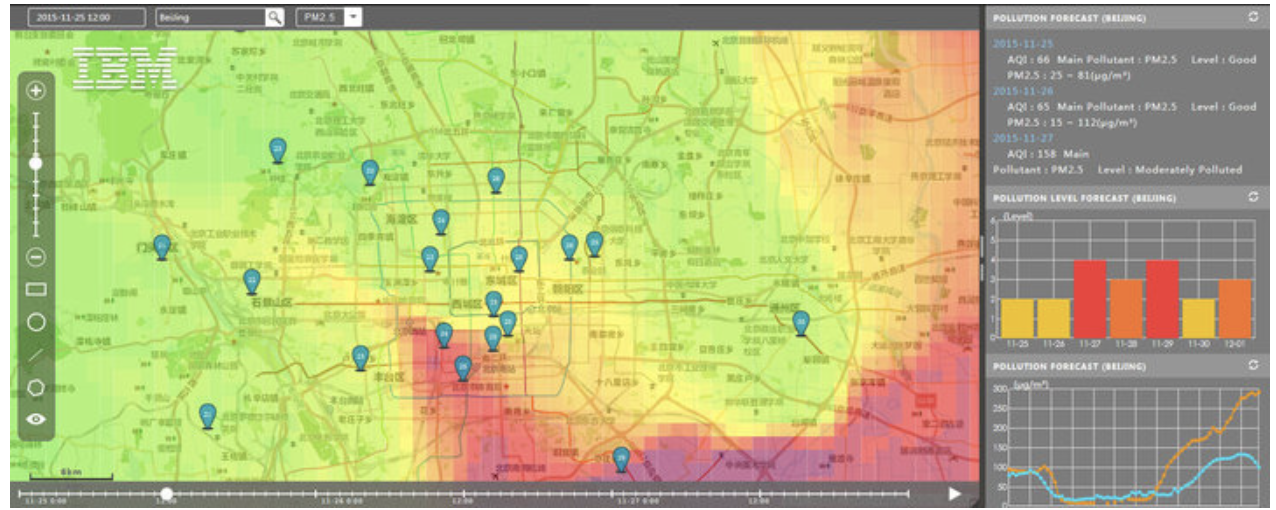
\includegraphics[width=0.7\textwidth]{images/fig1.png}
\caption{Truth Discovery In Data Streams \cite{Zhao2014}}
\end{figure}

\subsection{Evidence Based Approaches}


\section{Real-time Fact Checking}


\subsection{ClaimBuster}
 

\begin{figure}
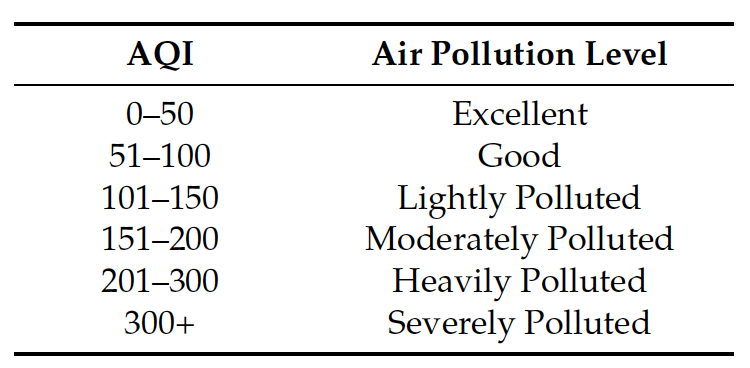
\includegraphics[width=0.7\textwidth]{images/fig2.png}
\caption{System architecture of ClaimBuster \cite{Claimbuster2017}}
\end{figure}

\section{Conclusion}

    
\begin{acks}

The author would like to thank Dr. Gregor von Laszewski and the teaching assistants for their support and suggestions in writing this paper.

\end{acks}

\bibliographystyle{ACM-Reference-Format}
\bibliography{report} 

\end{document}
